\documentclass{llncs}
\usepackage{amssymb}
\usepackage{graphicx}
\usepackage[ruled,linesnumbered,boxed]{algorithm2e}
\usepackage{graphicx}
\usepackage{amsmath}
\usepackage{bigstrut}
%\usepackage{mathtools}
%\usepackage{color}
\usepackage{tabularx}
\usepackage[colorlinks, linkcolor=blue, anchorcolor=blue, citecolor=green]{hyperref}
%\usepackage{booktabs}
\usepackage[table]{xcolor}
%\uespackage{colortbl}
\usepackage[tight,footnotesize]{subfigure}
\usepackage{fancyhdr}
\usepackage{lastpage}
\usepackage{layout}
%\usepackage{ctex}

%\footskip = 10pt
\pagestyle{fancy}
\chead{Group Project}
\lhead{CS214-Algorithm@SJTU}
\rhead{Instructor: Xiaofeng Gao}
\rfoot{}
\cfoot{Page \thepage \ of \pageref{LastPage}}
\addtolength{\headheight}{0.5\baselineskip}
\addtolength{\headwidth}{0\marginparsep}
\addtolength{\headwidth}{0\marginparwidth}

\title{Task Scheduling among Geographically Distributed Datacenters with Max-min Fairness}
\subtitle{A Stage-Wide Approach Based on Network Flow\vspace{-3mm}}

\author{Wendi Chen (519021910071, chenwendi-andy@sjtu.edu.cn)\\Wenhao Chen (519030910217, cccwher@sjtu.edu.cn)\\Haoyi You(519030910193, yuri-you@sjtu.edu.cn)}
\institute{Department of Computer Science, \\ Shanghai Jiao Tong University, Shanghai, China}

\begin{document}
\bibliographystyle{splncs}

%\linespread{0.85}

%==============================================================================
\maketitle

\begin{abstract}\vspace{-5mm}
In this paper, we focus on solving multi-job scheduling problem among geographically distributed data centers. We design different algorithms to assign tasks of jobs to datacenters based on the execute time, resource transmit time and dependence among them, in order to get minimal finishing time.

Unfortunately, this problem is proved to be a NP-Complete problem, which indicates the difficulty of finding the optimal solution in polynomial time. Thus, we divide the problem into many stages so that we can apply our algorithms to some dependency-free tasks in each stage to obtain a approximate optimal solution.

We first propose some greedy based algorithms, they are \textbf{Greedy Approach},\textbf{K-Greedy Approach} and \textbf{Network-Flow-Based Greedy Approach}.

Then, we focus on the max-min fairness of the solution. and propose \textbf{Network-Flow-Based Fair Approach} to achieve this.

Finally, we compare the performance of all these algorithms. To better understand the difference between them, we implement a data generator and compare the performance of them under numerous data instances.

\textbf{Keywords:} \textbf{multi-job scheduling problem, max-min fairness, Network-Flow Based Algorithm}.
\end{abstract}
\section{Introduction}
Nowadays, there are countless bytes of data generated every second. In order to make best use of these data, we build datacenters (DC) which are distributed across the world and process data by running data analytic jobs in the slots of DCs. Thus, we need to design a strategy to arrange these jobs to minimize the overall run time so that the throughput of the whole system can be optimized. However, to solve this problem, we will encounter several challenges as below.
\begin{enumerate}
    \item Each job is composed of several computation stages among which there are precedence constraints, which can be described in a directed acyclic graph (DAG). As a result, the tasks in different stages can not be arranged simultaneously. Also, the arrangement of the previous step may influence the available slots and arrangement of the next stage.
    \item The data on which one job depends are geographically dispersed and the bandwidth between two DCs is limited. In addition, the topology of the network is not necessarily fully connected, which means data should be transmitted between DCs.
    \item The number of slots in each DC is limited, which means tasks may have to wait after it is ready for running.
    \item In addition to minimize the average completion time of all jobs, we have to maintain \emph{max-min fairness}. However, these two optimization objectives are in contradictory to some extend.
\end{enumerate}

To address these challenges, we designed a multi-module scheduling model (Fig. \ref{Fig-Flowchart}), which consists of a DAG scheduler, a dependency-free task scheduler and a simulator to emulate a real production environment with multiple DCs. Our overall strategy is stage-wide greedy, i.e. we keep the average completion time of each stage as short as possible to make the total completion time as short as possible. Here, we use the DAG scheduler to get the tasks for each stage which are dependency-free. To achieve a fair scheduling algorithm, Chen \emph{et al.} \cite{LP-paper} have proposed a linear-programming-based approach. We extract the core idea from it and give a network-flow-based approach to achieve similar results.
\begin{figure}
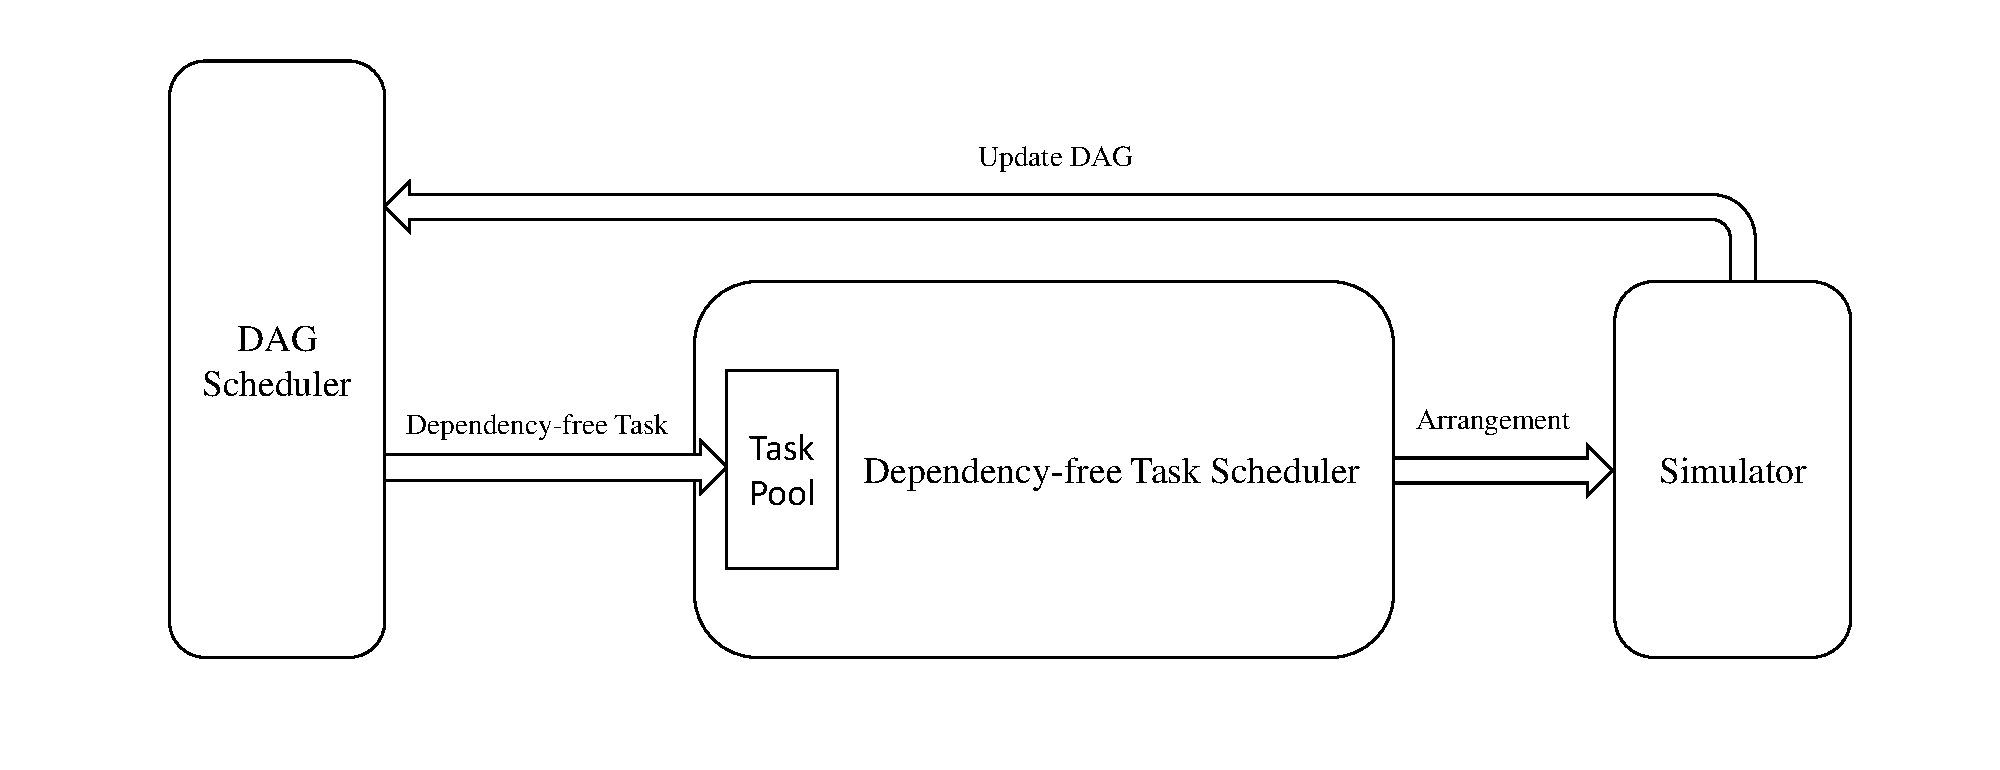
\includegraphics[width=0.8\textwidth]{figure/Fig-FlowChart.pdf}
\centering
\caption{Flowchart of the Model} \label{Fig-Flowchart}
\end{figure}
% \subsection{A Subsection Sample}
Please note that the first paragraph of a section or subsection is
not indented. The first paragraph that follows a table, figure,
equation etc. does not need an indent, either.

Subsequent paragraphs, however, are indented.

\subsubsection{Sample Heading (Third Level)} Only two levels of
headings should be numbered. Lower level headings remain unnumbered;
they are formatted as run-in headings.

\paragraph{Sample Heading (Fourth Level)}
The contribution should contain no more than four levels of
headings. Table~\ref{tab1} gives a summary of all heading levels.

\begin{table}
\caption{Table captions should be placed above the
tables.}\label{tab1}
\centering
\begin{tabular}{|l|l|l|}
\hline
Heading level &  Example & Font size and style\\
\hline
Title (centered) &  {\Large\bfseries Lecture Notes} & 14 point, bold\\
1st-level heading &  {\large\bfseries 1 Introduction} & 12 point, bold\\
2nd-level heading & {\bfseries 2.1 Printing Area} & 10 point, bold\\
3rd-level heading & {\bfseries Run-in Heading in Bold.} Text follows & 10 point, bold\\
4th-level heading & {\itshape Lowest Level Heading.} Text follows & 10 point, italic\\
\hline
\end{tabular}
\end{table}

\noindent Displayed equations are centered and set on a separate
line.
\begin{equation}
x + y = z
\end{equation}
Please try to avoid rasterized images for line-art diagrams and
schemas. Whenever possible, use vector graphics instead (see
Fig.~\ref{fig1}).

\begin{figure}
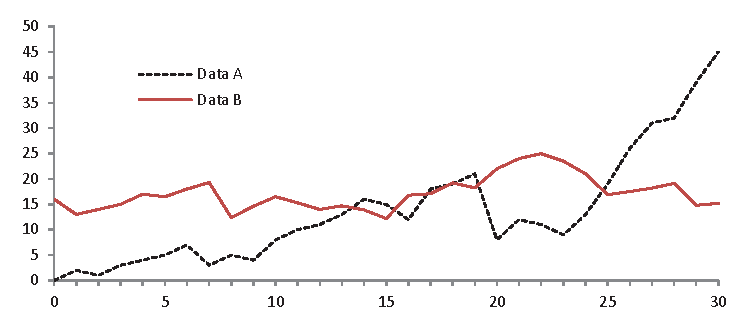
\includegraphics[width=0.6\textwidth]{figure/fig1.eps}
\centering
\caption{A figure caption is always placed below the illustration.
Please note that short captions are centered, while long ones are
justified by the macro package automatically.} \label{fig1}
\end{figure}

\begin{theorem}
This is a sample theorem. The run-in heading is set in bold, while
the following text appears in italics. Definitions, lemmas,
propositions, and corollaries are styled the same way.
\end{theorem}
%
% the environments 'definition', 'lemma', 'proposition', 'corollary',
% 'remark', and 'example' are defined in the LLNCS documentclass as well.
%
\begin{proof}
Proofs, examples, and remarks have the initial word in italics,
while the following text appears in normal font.
\end{proof}
For citations of references, we prefer the use of square brackets
and consecutive numbers. Citations using labels or the author/year
convention are also acceptable. The following bibliography provides
a sample reference list with entries for journal
articles~\cite{ref_article1}, an LNCS chapter~\cite{ref_lncs1}, a
book~\cite{ref_book1}, proceedings without editors~\cite{ref_proc1},
and a homepage~\cite{ref_url1}. Multiple citations are grouped
\cite{ref_article1,ref_lncs1,ref_book1},
\cite{ref_article1,ref_book1,ref_proc1,ref_url1}.
\section{Assumptions and Problem Analysis }
\subsection{Notations}
We use the similar notations in \cite{LP-paper} to describe task scheduling problem (Tab. \ref{tab-notation}). 
\begin{table}[htb]
\caption{Notations Used to Formulate Task Scheduling Problem}\label{tab-notation}
\centering
\begin{tabular}{|c|c|}
\hline
Notation & Meaning  \\
\hline
$\mathcal{K}$ & set of jobs \\
$J$&  set of DCs with idle slots \\
$\mathcal{T}_k$ & set of tasks of job $k$ \\
$S_i^k$ & set of source DCs of task $i$ of job $k$ \\
$R_i^k$ & set of the task $q$ of job $k$ which provides data required by task $i$ of job $k$\\
$a_j$ & the number of slots in DC $j$\\
$b_{s,j}$ & the band width from DC $s$ to DC $j$\\
$c_{i,j}^k$ & the data transferring time of task $i$ of job $k$ when it is assigned to DC $j$\\
$d_{i}^{k,s}$ & the amount of data in DC $s$ required by task $i$ of job $k$\\
$e_{i,j}^k$ & the data executing time of task $i$ of job $k$ \\
$s_i^k$ & the time when task $i$ of job $k$ is assigned to a slot\\
$f_i^k$ & the completion time of task $i$ of job $k$\\
$\tau_k$ & completion time of job $k$\\
$x_{i,j}^k$ & whether task $i$ of job $k$ is assigned to DC $j$\\
\hline
\end{tabular}
\end{table}


\subsection{Assumption}

\begin{enumerate}
    \item If there are idle slots in DCs and waiting tasks in ready queue, it would be better to assign tasks to idle slots. In other words, the bandwidth between different DC should not differ too much, so that it is better to wait some DC with higher bandwidth than transferring data to others.
    \item As DCs are not fully-connected, we implement Floyd Algorithm to compute the bandwidth between any DC pairs. Here new bandwidth is the lowest bandwidth along the path. Floyd transition function is  
    \begin{equation*}
        b_{i,j}=\max_{k\in V} \{ \min\{b_{i,k},b_{k,j}\} \}
    \end{equation*}
    
    \item Bandwidths are independent to tasks. That is, different tasks do not share bandwidth when transferring simultaneously.  
\end{enumerate}
\section{Assumptions and Problem Analysis }
\subsection{Notations}
We use the similar notations in \cite{LP-paper} to describe task scheduling problem (Tab. \ref{tab-notation}). 
\input{table/table-notation}


\subsection{Assumption}

\begin{enumerate}
    \item If there are idle slots in DCs and waiting tasks in ready queue, it would be better to assign tasks to idle slots. In other words, the bandwidth between different DC should not differ too much, so that it is better to wait some DC with higher bandwidth than transferring data to others.
    \item As DCs are not fully-connected, we implement Floyd Algorithm to compute the bandwidth between any DC pairs. Here new bandwidth is the lowest bandwidth along the path. Floyd transition function is  
    \begin{equation*}
        b_{i,j}=\max_{k\in V} \{ \min\{b_{i,k},b_{k,j}\} \}
    \end{equation*}
    
    \item Bandwidths are independent to tasks. That is, different tasks do not share bandwidth when transferring simultaneously.  
\end{enumerate}
\section{Assumptions and Problem Analysis }
\input{file/Model and Formulation/notations}
\input{file/Problem Analysis/Assumption.tex}
\input{file/Problem Analysis/Problem Analysis.tex}
\input{file/Model and Formulation/Notations of the Original Problem}
\input{file/Model and Formulation/Notations of the Sub-problem}



\subsection{Notations of the Original Problem}
In order to formulate the original problem, we need to give the corresponding notations. We assume that we now have a set of jobs in the $\mathcal{K} = \{1,2,\cdots,K\}$ to schedule. There are $J$ DCs which are denoted by $\mathcal{D} = \{1,2,\cdots,J\}$ and the number of slots in DC $j\in\mathcal{D}$ is $a_j$. Besides, each job $k\in\mathcal{K}$ has a set of tasks $\mathcal{T}_k = \{1,2,\cdots,n_k\}$. The set of the source DCs of task $i$ of job $k$ is $S_i^k$ and the set of the task $q$ of job $k$ which provides data required by task $i$ of job $k$ is $R_i^k$. If the source DC is $s$, the corresponding amount of data is $d_i^{k,s}$. Then, we denote the data transferring time and executing time of task $i$ of job $k$ when it is assigned to DC $j$ as $c_{i,j}^k$ and $e_{i,j}^k$ respectively and the bandwidth from DC $s$ to DC $j$ is $b_{s,j}$. From our previous assumption, we have
\begin{equation}
    c_{i,j}^k = \max_{s\in S^k_i} \frac{d_{i}^{k,s}}{b_{s,j}}
\end{equation}

If we define $x_{i,j}^k$ that indicates whether task $i$ of job $k$ is assigned to DC $j$ and $s_i^k$ as the time task $i$ of job $k$ is put into the slot, we have the completion time of task $i$ of job $k$ is
\begin{equation}
    f_i^k = s_i^k+ \sum_{j\in \mathcal{D}} x_{i,j}^k(c_{i,j}^k+e_{i,j}^k)
\end{equation}

And the completion time of job $k$ is
\begin{equation}
    \tau_k = \max_{i\in\mathcal{T}_k} f_i^k
\end{equation}

One task can be assigned to one and only one DC and each DC has limited slots at any time $t$, so we can derive an optimization problem where $\text{[   ]}$ is defined as a boolean function which is 1 if the inside statement is true and otherwise 0.
\begin{align}
        \textbf{lexmin}_{x} \quad& \mathbf{f} = (\tau_1,\tau_2,\cdots,\tau_k)\\
    s.t. \quad & \tau_k = \max_{i\in\mathcal{T}_k} f_i^k,\forall k\in\mathcal{K}\\
    & f_i^k = s_i^k+ \sum_{j\in \mathcal{D}} x_{i,j}^k(c_{i,j}^k+e_{i,j}^k), \forall i \in \mathcal{T}_k,\forall k \in \mathcal{K}\\
    &\sum_{k\in\mathcal{K}}\sum_{i\in\mathcal{T}_k} x_{i,j}^k[s_i^k\le t< f_i^k]\le a_j, \forall j \in \mathcal{D}, \forall t\ge 0\\
    & f_q^k\le s_i^k, \forall q\in R_i^k,\forall i \in \mathcal{T}_k,\forall k \in \mathcal{K}\\
    &\sum_{j\in\mathcal{D}}x_{i,j}^k = 1,\forall i \in\mathcal{T}_k,\forall k\in\mathcal{K}\\
    & x_{i,j}^k \in \{0,1\}, \forall i \in \mathcal{T}_k,\forall{j}\in\mathcal{D},\forall k \in \mathcal{K}
\end{align}

According to the definition of \emph{lexmin}, we can solve this optimization problem using the algorithm in (\ref{max-min}) to maintain max-min fairness.
% \newpage

\subsection{Notations of the Sub-problem}
\label{sub-problem}
In order to formulate the sub-problem, we need to give the corresponding notations. We assume that we now have a set of parallel jobs in the task pool $\mathcal{K} = \{1,2,\cdots,K\}$ to schedule. There are $J$ DCs which are denoted by $\mathcal{D} = \{1,2,\cdots,J\}$ and the number of idle slots in DC $j\in\mathcal{D}$ is $a_j$. Besides, each job $k\in\mathcal{K}$ has a set of tasks $\mathcal{T}_k = \{1,2,\cdots,n_k\}$. The set of the source DCs of task $i$ of job $k$ is $S_i^k$. If the source DC is $s$, the corresponding amount of data is $d_i^{k,s}$. Then, we denote the data transferring time and executing time of task $i$ of job $k$ when it is assigned to DC $j$ as $c_{i,j}^k$ and $e_{i,j}^k$ respectively and the bandwidth from DC $s$ to DC $j$ is $b_{s,j}$. From our previous assumption, we have
\begin{equation}
    c_{i,j}^k = \max_{s\in S^k_i} \frac{d_{i}^{k,s}}{b_{s,j}}
\end{equation}

If we define $x_{i,j}^k$ that indicates whether task $i$ of job $k$ is assigned to DC $j$, because every task of one job are dependency-free, we have the completion time of job $k$ is
\begin{equation}
    \tau_k = \max_{i\in\mathcal{T}_k,j\in \mathcal{D}} x_{i,j}^k(c_{i,j}^k+e_{i,j}^k)
\end{equation}

One task can be assigned to one and only one DC and each DC has limited slots, so we can derive an optimization problem where $lexmin$ is defined in \cite{LP-paper}.
\begin{align}
    \textbf{lexmin}_{x} \quad& \mathbf{f} = (\tau_1,\tau_2,\cdots,\tau_k)\\
    s.t. \quad & \tau_k = \max_{i\in\mathcal{T}_k,j\in \mathcal{D}} x_{i,j}^k(c_{i,j}^k+e_{i,j}^k),\forall k\in\mathcal{K}\\
    &\sum_{k\in\mathcal{K}}\sum_{i\in\mathcal{T}_k} x_{i,j}^k\le a_j, \forall j \in \mathcal{D}\\
    &\sum_{j\in\mathcal{D}}x_{i,j}^k = 1,\forall i \in\mathcal{T}_k,\forall k\in\mathcal{K}\\
    & x_{i,j}^k \in \{0,1\}, \forall i \in \mathcal{T}_k,\forall{j}\in\mathcal{D},\forall k \in \mathcal{K}
\end{align}

According to the definition of \emph{lexmin}, we can solve this optimization problem using the algorithm in (\ref{max-min}) to maintain max-min fairness.
% \newpage




\subsection{Notations of the Original Problem}
In order to formulate the original problem, we need to give the corresponding notations. We assume that we now have a set of jobs in the $\mathcal{K} = \{1,2,\cdots,K\}$ to schedule. There are $J$ DCs which are denoted by $\mathcal{D} = \{1,2,\cdots,J\}$ and the number of slots in DC $j\in\mathcal{D}$ is $a_j$. Besides, each job $k\in\mathcal{K}$ has a set of tasks $\mathcal{T}_k = \{1,2,\cdots,n_k\}$. The set of the source DCs of task $i$ of job $k$ is $S_i^k$ and the set of the task $q$ of job $k$ which provides data required by task $i$ of job $k$ is $R_i^k$. If the source DC is $s$, the corresponding amount of data is $d_i^{k,s}$. Then, we denote the data transferring time and executing time of task $i$ of job $k$ when it is assigned to DC $j$ as $c_{i,j}^k$ and $e_{i,j}^k$ respectively and the bandwidth from DC $s$ to DC $j$ is $b_{s,j}$. From our previous assumption, we have
\begin{equation}
    c_{i,j}^k = \max_{s\in S^k_i} \frac{d_{i}^{k,s}}{b_{s,j}}
\end{equation}

If we define $x_{i,j}^k$ that indicates whether task $i$ of job $k$ is assigned to DC $j$ and $s_i^k$ as the time task $i$ of job $k$ is put into the slot, we have the completion time of task $i$ of job $k$ is
\begin{equation}
    f_i^k = s_i^k+ \sum_{j\in \mathcal{D}} x_{i,j}^k(c_{i,j}^k+e_{i,j}^k)
\end{equation}

And the completion time of job $k$ is
\begin{equation}
    \tau_k = \max_{i\in\mathcal{T}_k} f_i^k
\end{equation}

One task can be assigned to one and only one DC and each DC has limited slots at any time $t$, so we can derive an optimization problem where $\text{[   ]}$ is defined as a boolean function which is 1 if the inside statement is true and otherwise 0.
\begin{align}
        \textbf{lexmin}_{x} \quad& \mathbf{f} = (\tau_1,\tau_2,\cdots,\tau_k)\\
    s.t. \quad & \tau_k = \max_{i\in\mathcal{T}_k} f_i^k,\forall k\in\mathcal{K}\\
    & f_i^k = s_i^k+ \sum_{j\in \mathcal{D}} x_{i,j}^k(c_{i,j}^k+e_{i,j}^k), \forall i \in \mathcal{T}_k,\forall k \in \mathcal{K}\\
    &\sum_{k\in\mathcal{K}}\sum_{i\in\mathcal{T}_k} x_{i,j}^k[s_i^k\le t< f_i^k]\le a_j, \forall j \in \mathcal{D}, \forall t\ge 0\\
    & f_q^k\le s_i^k, \forall q\in R_i^k,\forall i \in \mathcal{T}_k,\forall k \in \mathcal{K}\\
    &\sum_{j\in\mathcal{D}}x_{i,j}^k = 1,\forall i \in\mathcal{T}_k,\forall k\in\mathcal{K}\\
    & x_{i,j}^k \in \{0,1\}, \forall i \in \mathcal{T}_k,\forall{j}\in\mathcal{D},\forall k \in \mathcal{K}
\end{align}

According to the definition of \emph{lexmin}, we can solve this optimization problem using the algorithm in (\ref{max-min}) to maintain max-min fairness.
% \newpage

\subsection{Notations of the Sub-problem}
\label{sub-problem}
In order to formulate the sub-problem, we need to give the corresponding notations. We assume that we now have a set of parallel jobs in the task pool $\mathcal{K} = \{1,2,\cdots,K\}$ to schedule. There are $J$ DCs which are denoted by $\mathcal{D} = \{1,2,\cdots,J\}$ and the number of idle slots in DC $j\in\mathcal{D}$ is $a_j$. Besides, each job $k\in\mathcal{K}$ has a set of tasks $\mathcal{T}_k = \{1,2,\cdots,n_k\}$. The set of the source DCs of task $i$ of job $k$ is $S_i^k$. If the source DC is $s$, the corresponding amount of data is $d_i^{k,s}$. Then, we denote the data transferring time and executing time of task $i$ of job $k$ when it is assigned to DC $j$ as $c_{i,j}^k$ and $e_{i,j}^k$ respectively and the bandwidth from DC $s$ to DC $j$ is $b_{s,j}$. From our previous assumption, we have
\begin{equation}
    c_{i,j}^k = \max_{s\in S^k_i} \frac{d_{i}^{k,s}}{b_{s,j}}
\end{equation}

If we define $x_{i,j}^k$ that indicates whether task $i$ of job $k$ is assigned to DC $j$, because every task of one job are dependency-free, we have the completion time of job $k$ is
\begin{equation}
    \tau_k = \max_{i\in\mathcal{T}_k,j\in \mathcal{D}} x_{i,j}^k(c_{i,j}^k+e_{i,j}^k)
\end{equation}

One task can be assigned to one and only one DC and each DC has limited slots, so we can derive an optimization problem where $lexmin$ is defined in \cite{LP-paper}.
\begin{align}
    \textbf{lexmin}_{x} \quad& \mathbf{f} = (\tau_1,\tau_2,\cdots,\tau_k)\\
    s.t. \quad & \tau_k = \max_{i\in\mathcal{T}_k,j\in \mathcal{D}} x_{i,j}^k(c_{i,j}^k+e_{i,j}^k),\forall k\in\mathcal{K}\\
    &\sum_{k\in\mathcal{K}}\sum_{i\in\mathcal{T}_k} x_{i,j}^k\le a_j, \forall j \in \mathcal{D}\\
    &\sum_{j\in\mathcal{D}}x_{i,j}^k = 1,\forall i \in\mathcal{T}_k,\forall k\in\mathcal{K}\\
    & x_{i,j}^k \in \{0,1\}, \forall i \in \mathcal{T}_k,\forall{j}\in\mathcal{D},\forall k \in \mathcal{K}
\end{align}

According to the definition of \emph{lexmin}, we can solve this optimization problem using the algorithm in (\ref{max-min}) to maintain max-min fairness.
% \newpage




\section{NP-Completeness of Problem}\label{section:npc}

\subsection{Brief Introduction}
In order to prove this problem to be an NP-Complete problem, we need to introduction 3 new problems,\\$\textbf{P1,P2,P3}$.
\begin{enumerate}
    \item $\textbf{P1}~\emph{Single Execution Time Scheduling}:$ \\ 
    Given a set $\mathbb{S}$ of $n$ tasks, a partial order $\prec$ on $\mathbb{S}$,  a number of processors $k$ and a time limit $t$, does there exist 
    a total function $\mathbf{f}$ from $\mathbb{S}$ to $\{0, 1,..., t - 1\}$ such that
    \begin{enumerate}
        \item if $J\prec J'$ then  $f(J)+1\le f(J')$.
        \item for each $J$ in $\mathbb{S}$, $f(J)  \le t-1$.
        \item for each $i, 0\le i< t$, there are at most $k$ values of $J$ for which $f(J)=i$.
    \end{enumerate}
    \item $\textbf{P2}~\emph{Single Execution Time Scheduling with variable number of processors}:$ \\ 
    Given a set $\mathbb{S}$ of $n$ tasks, a partial order $\prec$ on $\mathbb{S}$, a time limit $t$ and a sequences of integers$\{c_0,c_1\dots c_{t-1}\}$satisfies $\sum\limits_{i=0}^{t-1}c_i=n$ represents the number of processors in every time, does there exist 
    a total function $\mathbf{f}$ from $\mathbb{S}$ to $\{0, 1,..., t - 1\}$ such that
    \begin{enumerate}
        \item if $J\prec J'$ then  $f(J)+1\le f(J')$.
        \item for each $J$ in $\mathbb{S}$, $f(J) \le t-1$.
        \item for each $i, 0\le i< t$, there are $c_i$ values of $J$ for which $f(J)=i$.
    \end{enumerate}
    % \item $\textbf{P1}~\emph{Single Execution Time Scheduling}:$ \\ 
    \item $\textbf{P3}~\emph{3-SAT}:$\\
    Given a set of literals $\mathbb{X}=\{x_i,\overline{x_i}\}, 1 \le i \le n,x_i=\neg\Bar{x_i}$ and a collection of clause
$C_t=x_j\vee x_k\vee x_l,1\le t\le n$ that satisfies $x_j,x_k,x_l=x_i~or~\Bar{x_i}$,does there exist a map $f$ from $\mathbb{X}$ to  $\{\textbf{True},\textbf{False}\}$ satisfies that $\forall t, C_t=\textbf{True}$. 
\end{enumerate}
 Then we prove $\textbf{P3}\preceq_p \textbf{P2}\preceq_p\textbf{P1}$.\\As for $\textbf{P1,P2}$,given an scheduling sequences, we can easily determine whether the result $\le t$, so $\textbf{P1,P2}$ are both NP problem. And since we have known $P3$ is an NP-Complete problem, we get $P1$ is also an NP-Complete problem.\\
 If we constrain the time of each task to be 1,the number of jobs to be 1 and do not need any resource(or transmit time to be 0) for problem $\textbf{P1}$.Then we know 123456 is an NP-Complete problem.
\subsection{Proof of $\textbf{P2}\preceq_p \textbf{P1}$}
As for given problem $\textbf{P2}$,we have $\mathbb{S}$ of $n$ jobs, limits $t$ and sequences $\{c_0,c_1\dots c_{t-1}\}$. Then we construct a new problem as $\textbf{P1}$.
\begin{enumerate}
    \item Let $n=\sum\limits_{k=0}^{t-1}c_k$
    \item Add new tasks $J_{i,j}$ with $0\le i\le t-1,0\le j\le n-c_i$ into $\mathbb{S}$.
    \item Add partial order to new tasks. For $\forall J_{i_1,j_1}, J_{i_2,j_2}$,if $i_1\le i_2$, then let $J_{i_1,j_1}\preceq J_{i_2,j_2}$.
    \item Let the number of processors to be $c$.
\end{enumerate}
Because of the constraint between new tasks, there are $t$ levels, so we must assign the $J_{i,j}$ at time $i$.Otherwise, assume $f(J_{i,j})=k$ and $i\neq k$,
\begin{enumerate}
    \item If $i>k$, assume $J_{i,j}$ be the earliest task that $i>k$, then $\exists J_{i-1,j'}$,from the assumption that $f(J_{i-1,j'})=i-1\ge k$. So $f(J_{i,j})\le f(J_{i-1,j'})$ which is against problem requirement.
    \item If $i<k$, assume $J_{i,j}$ be the latest  task that $i<k$, then there $\exists J_{i+1,j'}$,from the assumption that $f(J_{i+1,j'})=i-1\le k$. So $f(J_{i,j})\ge f(J_{i+1,j'})$ which is against problem requirement.
\end{enumerate}
Then after we assign all new tasks, the remain processors at time $i$ is $n-(c-c_i)=c_i$,so there are at most $c_i$ values of $J$ for which $f(J)=i$. However,$\sum\limits_{i=0}^{t-1}c_i=n$, which means we must assign $c_i$ tasks at time $i$,otherwise we cannot finish all tasks at time $t$.As a result, there are $c_i$ values of $J$ for which $f(J)=i$,so the new problem is a $\textbf{P1}$ problem,and the original and new problem are equal.
\subsection{Proof of $\textbf{P3}\preceq_p \textbf{P2}$}
As for given problem $\textbf{P3}(\emph{3-SAT})$, assume there are $m$ variables($2m$ literals)$\{x_i,\overline{x_i}\}$ and $n$ clauses $\{D_j\}$.We construct a new problem as $\textbf{P2}$.
\begin{enumerate}
    \item Task set $\mathbb{S}$.
    \begin{equation}
    \begin{aligned}
        \mathbb{S}~&=\mathbb{X'\cup Y'\cup D'}\\
        \mathbb{X'}&=\bigcup_{\substack{1\le i\le m\\ 1\le j\le m}}\{x_{i,j},\overline{x}_{i,j}\}\\
        \mathbb{Y'}&=\bigcup_{1\le i\le m}\{y_i,\overline{y}_i\}\\
        \mathbb{D'}&=\bigcup_{\substack{1\le i\le n\\ 1\le j\le 7}}\{D_{i,j}\}
    \end{aligned}
    \end{equation}
    \item Relation $\prec$\\
    \begin{enumerate}
        \item $x_{i,j}\prec x_{i,j+1}, \overline{x}_{i,j}\prec \overline{x}_{i,j+1}$,for $1\le i\le m, 1\le j\le m$.
        \item $x_{i,i-1}\prec y_{i},\overline{x}_{i,i-1}\prec \overline{y}_{i}$, for $1\le i\le m, 1\le j\le m$.
        % \item $y_{i-1}\prec y_{i},\overline{y_{i-1}}\prec \overline{y_{i}}$
        \item
        For a random literals $z_i=x_i~or~\overline{x_i}$ and a boolen value $a\in\{0,1\}$, we define 
        \begin{equation}
            \begin{aligned}
            a\odot z_i=\left\{\begin{array}{lr}
             z_i(=x_i~or~\overline{x_i})~~~~~~~~~~if~a=1\\
             \overline{z_i}(=\overline{x_i}~or~x_i)~~~~~~~~~~if~a=0\\
             \end{array}\right.
            \end{aligned}
        \end{equation}
         For task $D_{i,j}$, since $j\le 7$,assume $j=a_1*4+a_2*2+a_3,a_i\in\{0,1\},1\le i\le 3$. \\
        From the \textbf{3-SAT} problem, assume $D_i=z_{b_1}\vee z_{b_2}\vee z_{b_3}$ that $z_{b_k}=x_{b_k}~or~\overline{x_{b_k}}$. If $z_{b_k}=x_{b_k}$, let $z_{{b_k},j}$ refer to the task $x_{{b_k},j}$,else let $z_{{b_k},j}$ refer to the task $\overline{x}_{{b_k},j}$, $1\le k \le 3$\\
        Then we add relation $\prec$ that
        \begin{equation}
            a_{k}\odot z_{{b_k},m}\prec D_{{b_k},j}. 1\le k \le 3.
        \end{equation}
    \end{enumerate}
        \item The time limit is $m+3$.
        \item The sequences $\{c_i\}(0\le i\le m+2)$ of processors limits
        \begin{equation}
            \begin{aligned}
            c_i&=2m+2~~~~~~~~~~~~2\le i \le m\\
            c_0&=m~~~~~~~~~~~~~~~~~c_1=2m+1\\
            c_{m+1}&=n+m+1~~~~~~~c_{m+2}=6n
            \end{aligned}
        \end{equation}
\end{enumerate}
Here we prove the problem constructed above is equal to the given $\textbf{3-SAT}$ problem.\\
    Exactly, we only need to prove for above problem, there exists 
    a total function $\mathbf{f}$ from $\mathbb{S}$ to $\{0, 1,..., m+2\}$ that satisfies the condition $\Leftrightarrow$ for each $D_i=D_i=z_{b_1}\vee z_{b_2}\vee z_{b_3}$, at least one of the literals $z_{b_k}$, $f(z_{b_k,0})=0$.Then if $z_{b_k,0}=0$,in $\textbf{P3}$, let $z_{b_k}=\textbf{True}$,so for each clause, $D_i=\textbf{True}$.\\
    To prove this, we have several steps.\\
    Firstly, we may not execute both $x_{i,0}$ and $\overline{x}_{i,0}$ at time $0,1\le i\le m$. Assume $\exists i,f(x_{i,0})=f(\overline{x}_{i,0})=0$. Since $c_0=m$, there exists $j$ that $f(x_{i,0})=f(\overline{x}_{i,0})\ge 1$, which means $f(y_i)>j$  and $f(\overline{y_i})>j$. Then we count the maximum number of tasks $z$ that $f(z)\le j$, which is consist of two parts:
    \begin{enumerate}
        \item For every $z_i$.If $f(z_{i,0})$,there are $z_{i,0}\dots z_{i,j}$, else there are $z_{i,0}\dots z_{i,j-1}$. Since there are at most $m$ of $z_i$ satisfies $f(z_{i,0})=1$, the total number of tasks $\le m*(2j+1)$.
        \item $y_1,\overline{y_1},\dots, y_{i-1},\overline{y_{i-1}}$, the total number $\le 2*(j-1)$.
    \end{enumerate}
    So the total number of tasks $\le m*(2j+1)+2*(j-1)=2mj+2j+m-1$. However,
    \begin{equation}
        \sum_{i=0}^{j}=2mj+2j+m-1\ge2mj+2j+m-2
    \end{equation}
    This is against the requirement that there are $c_i$ tasks executed at time $i$.\\
    Secondly,at time $1\le j\le m$, if $f(x_{i,0})=0$, we execute $x_{i,j}$,otherwise we execute $x_{i,j-1}$. Moreover, if $f(x_{i,0})=0$,we must execute $y_i$ at time $t$, otherwise we execute $y_i$ at time $t+1$.\\
    Thirdly, at time $m+1$, we need execute remain m number of $z_{i,m}$. Because $c_{m+1}=m+n+1$, we must execute $n$ of $D_{i,j}$, and the other $D_{i,j}$ must be executed at time $m+2$, otherwise we are not able to finish all the tasks by the end of $m+3$.\\
    Lastly,if $\exists D_i=z_{b_1}\vee z_{b_2}\vee z_{b_3}=\textbf{False}$, $z_{b_1}=z_{b_2}=z_{b_3}=\textbf{False}$, so $f(z_{b_1})>1,f(z_{b_2})>1,f(z_{b_3})>1$, which means we are not able to assign $D_i$ at time $t+1$.As a result, we cannot finish the task by the end of time $m+3$.\\
    From the above steps, we conclude that there exists a instance satisfies  $\textbf{3-SAT}\Leftrightarrow$ there exists a function $f$ from $\mathbb{S}$ to $\{0,1,\dots,m+2\}$ satisfies the above condition. In the end, we have already proved $\textbf{P3}\preceq_p \textbf{P2}$.
    
    

\section{Model and Algorithms}
Because we have proved that a  multi-job scheduling problem is a NPC problem, it may be extremely hard to find the optimal solution to the original problem. Thus, we need to transform this problem into a simpler one and take its solution as an acceptable but not necessarily optimal solution to the original problem. More specifically, why the original problem is difficult to solve is because there are dependencies between tasks and the number of slots may be smaller than the number of tasks to be scheduled. Thus, we can design a DAG scheduler to get dependency-free tasks and use a task pool to temporarily store the tasks when the number of slots is not sufficient. That is what we call \textbf{stage-wide greedy}. We find the optimal arrangement for each small ``stage'' to obtain an approximate global optimal solution. Here, how to assign dependency-free tasks when there is enough slots become an important sub-problem which has been described in \ref{sub-problem}.
\subsection{DAG Scheduler}
DAG scheduler extracts nodes with no in-node degree from the graph and submits them to the task pool. When it receives the finished tasks from simulator, it should update the DAG correspondingly. In fact, to realize these two functions, we just need to maintain the successor nodes and the in-node degrees of each node. When we need to update the DAG, we just need to decrement the in-node degree of the successor nodes of each finish task.

\textbf{Time Complexity.} Using amortized analysis, it is $O(1)$ for each task.
\subsection{Scheduling Algorithms}\label{schedule algorithm}


\textbf{Notations}.
\begin{enumerate}
    \item \textbf{Assignment}: one feasible assignment (i.e. assign one task to one slot)
    \item $m=\sum \left |  \mathcal{T}_{k} \right |$ denote the amount of all dependent-free tasks.
\end{enumerate}

\subsubsection{Greedy Approach}\label{Greedy Approach}
~

Greedy Approach stems from a very natural intuition that we can schedule tasks to the idle slots with the shortest data transferring time, so that the sum completion time of each job in this small ``stage'' is also relatively short. 


    

\textbf{Procedure}. Compute a feasible assignment with shortest time. Bring this assignment into effect and repeat until all slots are full or all tasks have been assigned.

\textbf{Time Complexity}. We use priority queue to compute assignment with shortest time in $O(\log (|J|m))$. Thus, the time complexity is $O(m\log (|J|m))$. 

However, the greedy approach does not take max-min fairness into consideration. That is to say, it may improve the performances of some tasks while worsen others to achieve a relatively short sum completion time, which contradicts a lot with max-min fairness.
\subsubsection{K-Greedy Approach}\label{k-Greedy Approach}
~

\input{figure/fig-greedy_eg.tex}

When invoking Greedy Approach, we only consider about the very first task. And this may worsen the data transferring time of other tasks. This is better illustrated with example Fig. \ref{greedy_eg}. Greedy Approach first considers tA1 then tA2 and results in case (a). However, it is obvious that case (b) is better in both sum completion time and maximal completion time. Here, we introduce a randomized greedy approach, which is called K-Greedy Approach.

\textbf{Procedure}.
K-Greedy Approach randomly generate $k\sim U(0,2)$ for every task. Every time we compute an assignment with shortest data transferring time, we check whether $k$ is 0. If $k>0$, we simply skip this assignment and decrease $k$ by 1.

        % \begin{minipage}[t]{0.8\textwidth}
        %       \begin{algorithm}[H]
        %           %\LinesNumbered
        %           \KwIn{$x$, $y$}
        %           \KwOut{$sign$}
        %           \BlankLine
        %           \caption{$K-Greedy$} \label{Greedy_algo}

        %           $computes\ all\ possible\ assignments\ and\ put\ into\ priority\ queue$\;
        %           $randomly\ generate \ array\ K$\;
        %           $cnt \leftarrow 0$\;
        %           \While{$cnt < task\  number$}
        %           {
        %               $find\ assignment\ with\ shortest\ transferring\ time$\;
        %               $task \leftarrow assignment.task$\;
        %               \If{$K[task]>0 $ }
        %               {
        %                   $K[task]\leftarrow K[task]-1$\;
        %               }
        %               \ElseIf{$task \ is\ not\ assigned$}
        %               {
        %                   $bring\ this\ assignment\ into\ effect$\;
        %                   $cnt\leftarrow cnt+1$\;
        %               }
        %           }
        %       \end{algorithm}
        %   \end{minipage}

\textbf{Time Complexity}.
It may need k more iterations. Thus, time complexity is $O(km\log (|J|m))$.

K-Greedy Approach is able to yield case (b) in Fig. \ref{greedy_eg}. However, as $k$ is randomly generated, its performance is not so stable. Worse still, it may make unnecessary concessions and worsen the performance. 


\subsubsection{Network-Flow-Based Greedy Approach}\label{NFBGA}
~

K-Greedy Approach is able to yield better solution sometimes, but with poor stability. This raises a natural question, can we find an approach to minimize the sum data transferring time of $k$ tasks without randomness? The answer is YES and we can use a network-flow-based algorithm to achieve this, which computes maximal flow while maintain minimal cost sum.

\textbf{Construction}. 
    We construct a weighted network graph $G=(V,E,s,t,c_e,w_e)$, where $c_e$ is the capacity of edge and $w_e$ is the cost of edge. When there is $f(e)$ flow in $e$, we will add $f(e) \cdot w_e$ to total cost.
    
\begin{enumerate}
    \item
        To begin with, $s$ is virtual source and it connects DC $i$ with $c_e=a_i$ and $w_e=0$. This ensures we can not assign more tasks into one DC than the amount of its idle slots.
    \item
        For each DC $i$, it has exactly $m$ edges.
        Each edge connects to one task, say task $i$ of job $k$, with $c_e=1$ and $w_e=c_{i,j}^k$.
        $c_e=1$ ensures each task can only be assigned once while $w_e$ indicates the cost of this assignment.
        This results in  $\left | J \right | \cdot m $ edges in total, which cover all possible assignments.
        Here, we denote these edges as \textbf{Assignment Edges}.
        
    \item
        Finally, $t$ is a virtual sink and every task connects to it with $c_e=1$ and $w_e$.
\end{enumerate}
    In Fig. \ref{fig-network_greedy}, (a) shows the network we construct and (b) shows the maximal flow with minimal cost of this network.
  
\input{figure/fig-network_greedy.tex}  

\textbf{Solve}. To solves maximal flow with minimal cost, we can apply Bellman-Ford Algorithm to find shortest (i.e. minimal cost sum) augmenting path each iteration. As the cost is minimized, we minimize the sum data transferring time of tasks counted in maximal flow. To get the final assignments, we check each \textbf{Assignment Edge}. If $f(e)=1$, then it indicates this assignment is chosen in maximal flow and we bring this assignment into effect.

\textbf{Time Complexity}. The network has $O(|J|+m)$ nodes and $O(\left | J \right | m)$ edges. Thus, the time complexity is $O(|J|^2m+|J|m^2) $.


\textbf{Example}. This is better illustrate with example in Fig. \ref{greedy_eg}. And Fig. \ref{fig-network_greedy} is the corresponding network graph we construct. If we apply Greedy Approach, it will first assign tA1 to DC1 and tA2 to DC2, which yields case (a) and a total data transferring time of $2+6=8$. However, if apply network-flow-based Greedy Approach to consider these two tasks simultaneously, we are able to get case (b) and a total data transferring time $3+3=6$.


\subsubsection{Network-Flow-Based Fair Approach}\label{NFBFA}
~

Network-Flow-Base Greedy Approach only ensures that the sum data transferring time of $k$ tasks is minimized. However, it does not achieve max-min fairness and may suffer from same problem as Greedy Approach. Here, we introduce a Network-Flow-Based Fair Approach, which can achieve max-min fairness.

\textbf{Construction}. We construct the network graph similar to Network-Flow-Based Greedy Approach. But take both data transferring time and execute time into consideration (i.e. $w_e=c^k_{i,j}+e^k_{i,j}$).  

\textbf{Solve}. To achieve max-min fairness, we need first to minimize $\max\{c^k_{i,j}+e^k_{i,j}\}$. It is quite hard to find the optimal solution. However, to certificate it is much easier.  

Let $\Delta$ denote the answer.
\begin{enumerate}
    \item \textbf{Certifier}. Given a $\Delta$, let $G(\Delta)$ be the subgraph of $G$ consisting of only edges with $w_e\leq \Delta$. Then, we compute maximal flow in $G(\Delta)$. If $f_{max}=m$, then it indicates we can assign all dependent-free tasks within bottleneck $\Delta$.
    
    \item \textbf{Search $\Delta$}. Since, we already have a certifier. The remaining work is to find $\Delta$. We can observe that $\Delta$ is monotonic. In other words, given $\Delta_{min}$, $\Delta \geq \Delta_{min}$ are feasible solutions while $\Delta < \Delta_{min} $ are not. Thus, we can use binary search to accelerate the search of $\Delta$.
    
    \item \textbf{Max-Min Fairness}. Once we find the bottleneck of some tasks, the corresponding job's finish time can be better. Thus, we can assign other tasks (denoted by $ \mathcal{T}^{'}_{k}$) in the same job more arbitrarily as long as they do not worsen bottleneck. To achieve this, for each task in $ \mathcal{T}^{'}_{k}$, we check every corresponding edge in network graph. 
    \begin{enumerate}
        \item  If $w_e> bottleneck$, we can not bring this assignment into effect or it would worsen bottleneck. Thus, we need to set $w_e^{'}=\infty$ to ensure this edge will not be chose. 
        \item  If $w_e\leq bottleneck$, we just do the opposite and set $w_e^{'}=0$. This ensures these assignments will not affect finding bottleneck of other jobs.
    \end{enumerate}
    Moreover, we bring bottleneck assignment into effect and decrease DC capacity accordingly.
    After updating the network graph, we repeat the procedure and find the bottleneck of next job. Finally this procedure finishes when we find bottleneck of each job.
    
\end{enumerate} 
    
\input{figure/fig-fair.tex}
    
\textbf{Time Complexity}.Certifier takes $O(|J|^2m+|J|m^2)$ and binary search takes $O(\log(\max\{c_e\}) )$. Beside, we need $|\mathcal{K}|$ iterations to find bottleneck in each job respectively. Thus, the time complexity of Network-Flow-Based Fair Approach is $O((|J|^2m+|J|m^2)\log (\max \{c_e\}) |\mathcal{K}|)$.

\textbf{Example}. To illustrate better how Network-Flow-Based Fair Approach achieve max-min fairness, we introduce a new example Fig. \ref{fig-fair}. Suppose after construct we have network graph (a). We apply Network-Flow-Based Fair Approach on this and (b) shows the result of first iteration. After first iteration, we find assigning tA1 to DC1 is the bottleneck with $w_e=5$. Thus, we assign tA1 to DC1 and update the network graph accordingly. (c) shows the new network graph, where edges of job A are either $0$ or $\infty$. We repeat the procedure again and this time we find assigning tB1 to DC1 is the bottleneck with $w_e=2$. As there are only 2 jobs and we find 2 bottlenecks, the algorithm terminates with max-min fairness solution (tA1,tA2,tB1)$=(5,4,2)$.
Note that Greedy Base Approach can never give this solution as $(5,2,3)$ minimize the sum completion time.
    


\section{Experiments}\label{Experiments}
\subsection{Analysis of Toy Data}\label{Toy Data}

\textbf{Property}. If every DC has $\infty$ slots, then Greedy Approach yields the optimal solution.

As the amount of slots is infinity, assign one task will never worsen the data transferring time of others tasks. Thus, we can assign each task to its optimal position and this results an optimal solution of all jobs. The property enables us to find the optimal solution of toy data. 

In fact, DCs in toy data have relatively large slots amount. Applying Greedy Approach on toy data exactly yields the optimal solution. Beside, Network-Flow-Based Greedy Approach and Network-Flow-Based Fair Approach also yields this optimal solution while K-Greedy may sometimes yields a better time.

\begin{figure}[htb]
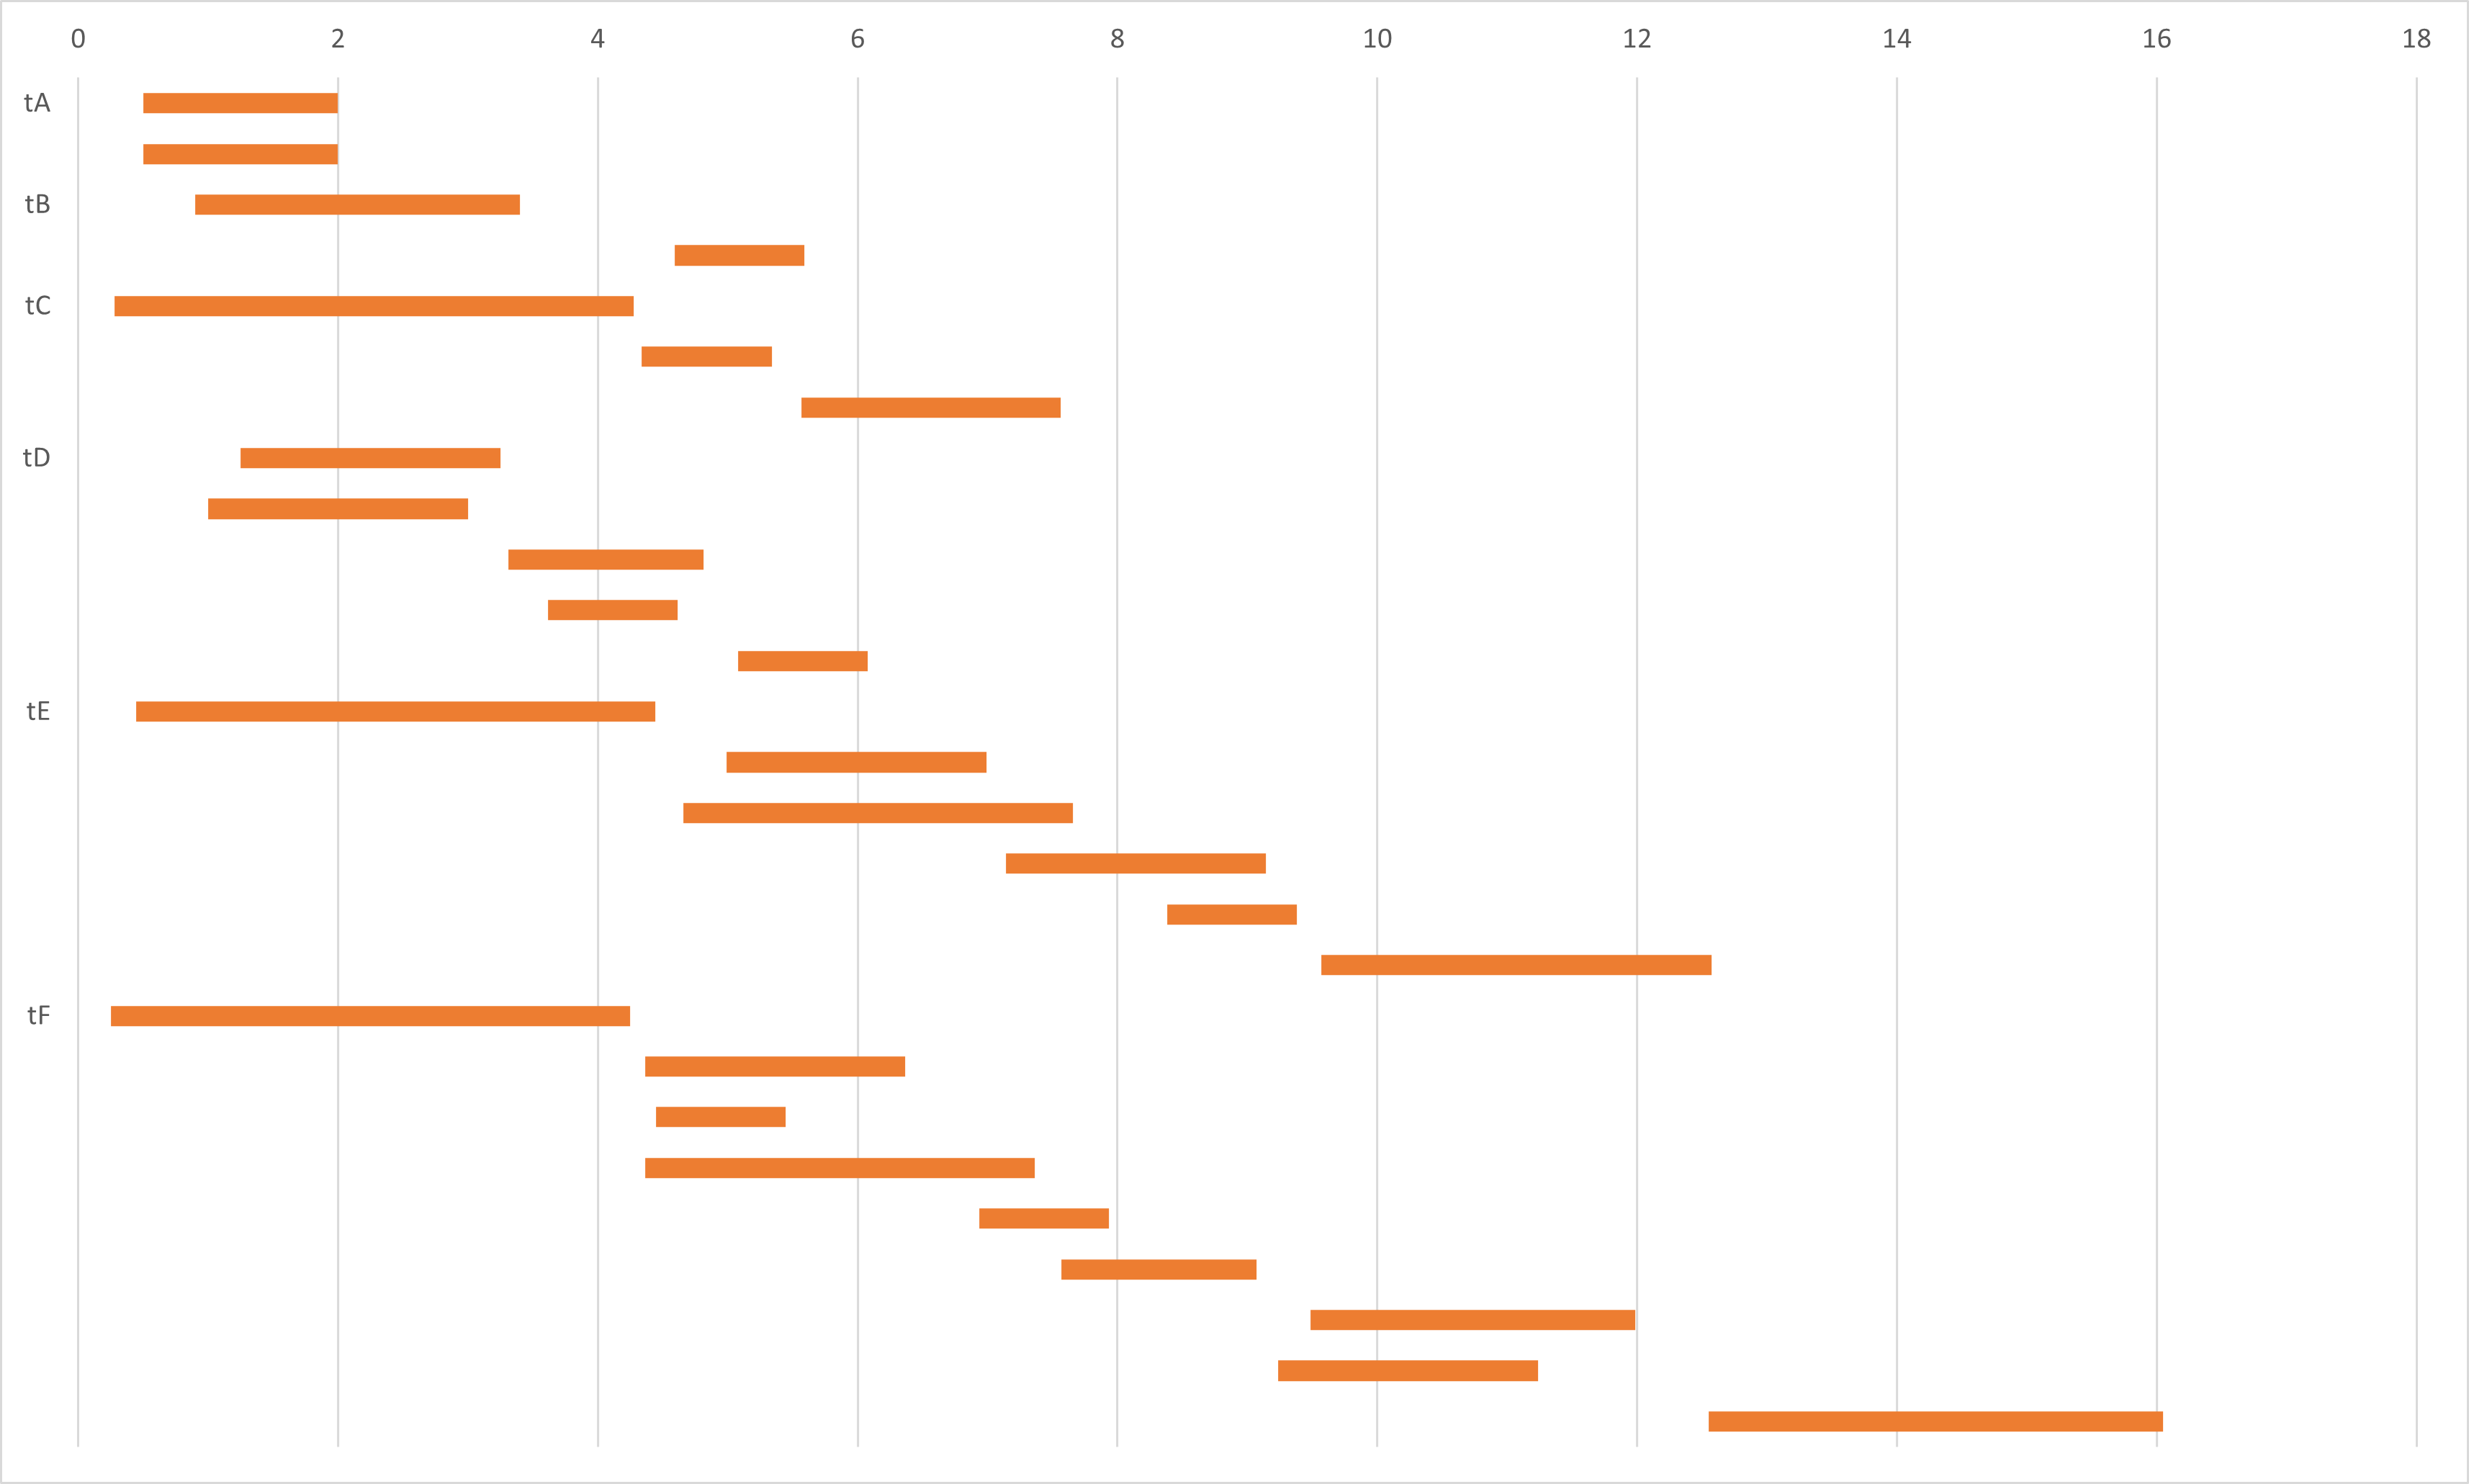
\includegraphics[width=0.8\textwidth]{figure/fig-toy.png}
\centering
\caption{Gantt chart of the optimal solution} \label{fig-toy}
\end{figure}

The solution is better illustrated by Fig. \ref{fig-toy}. The figure shows the start and finish time of each task.

\subsection{Data Generation and Performance Analysis}\label{data generator}
\subsubsection{Brief Introduction of Generator}
~\par
In order to make comparison with toy data, we do not modify the links between DCs. The whole generator is divided into three parts. First, for each job, a DAG composed of tasks is generated. Secondly, for each task, the data it depends on is generated. Finally, the data is distributed to each DC.
\subsubsection{Generator Implement Details}
~\par
To generate jobs, we should determined how many tasks each job has. From \cite{OSC}, we know that there are about 80\% jobs are short jobs and 20\% jobs are long jobs. For short jobs, the number of tasks $n\sim max(2,N(4,25))$. For long jobs, $n\sim max(10,N(20,100))$. Each job has an executing time $t\sim max(1,N(3,4))$.

After that, we generate DAG by numbering the nodes in the graph, and build an edge from a small number node to a large number node with a probability of 0.4. The larger number node will require more sets of data and the amount of one set of data required by each task in each DC $s\sim max(50,N(400,160000))$, which is basically consistent with the toy data. When assigning these data to DCs, we put the adjacent 4 data into one DC, which is easy to understand because the data used by one jobs should be centralized to some extent.

\subsubsection{Overview of The Performances}
~
\input{figure/60}

\input{figure/80}

We generate data with different job number and different proportion of small jobs. Fig. \ref{fig-60} and Fig. \ref{fig-80} show the maximal finish time, average finish time and its standard deviation.
We can observe the following outcome 
\begin{enumerate}
    \item Greedy and Fair Approach are much better than the random baseline. 
    \item K-Greedy Approach is not that stable but can sometimes yields a better solution.
    \item Greedy Approach and Network-Based Greedy have similar outcome.
    \item Network-Based Fair Approach have a high probability to achieve a best solutions in all metrics, with job amount and small job proportion are large.
\end{enumerate}

\subsubsection{Details Analysis of One Instance from Generator}
~\par
Based on the generator, we have tested lots of data and compare the performance of different algorithm. Data is random and different from time to time and we cannot show all of them in the paper, but most of them can reveal the similar performance of these algorithms, so we select one of the most representative data and analyse different performance of algorithms.To better analyse the performance, we introduce a random algorithm and regard the result of it as the baseline.
\begin{enumerate}
    \item Performances:~\par~\par
    \input{table/data analysis}
    ~\par~\par~\par
    \item Figures of the data. (Fig.\ref{fig-hist}, Fig.\ref{fig-residual})
    ~\par
    \input{figure/fig-hist}
    \input{figure/fig-residual}
    \item Results analysis:
    \begin{enumerate}
        \item Average time of the jobs:\\
        Comparing to the baseline, all of the algorithms have optimized the running time of each jobs and tasks. However, for most of time, the average time of different algorithms have no distinct different. That's because the targets of all algorithms are all to optimize the total time rather than forcing on certain tasks.
        \item Maximal finish time of the jobs:\\
        As for the finish time, Network-Flow-Based algorithms usually get more optimal and stable results, and the fair approach is always better than the other one, because it focus on the bottleneck of scheduling methods.\\
        However, the greedy approach algorithms are much more unstable. Sometimes the results will be very slow,even larger than the baseline(such as the K-greedy in this instance), while in other times these algorithms will reach a better performance(such as the toy data). Moreover, the K-greedy is more unstable than basic greedy algorithm.\\
        The results above is very nature. Greedy has much more possibility to be limited by the slots capacity bottleneck. If the slots capacity is further large,the greedy algorithm has larger chance to get better solutions.(If the capacity$=\infty$, this algorithm will get optimal solution.) However, if the slots capacity limits is tight, we must allocate the slots capacity globally. Thus greedy algorithms will result in a bad solution.
        \item Standard Deviation:\\
        Obviously, the Network-Flow-Based Fair Approach always reaches the least deviation. It is also easy to understand the result because in this algorithm we aim at the max-min fairness.This is also reflected on the results in Histogram (Fig.\ref{fig-hist}).
    \end{enumerate}
    \item Max-min Fairness of the Network-Flow-Based Fair Approach Algorithm:
    \begin{enumerate}
        \item Deviation in the this algorithm is always the least. This is because in this algorithm we minimize the maximal job and the jobs time becomes more concentrated.
        \item In residual Fig.\ref{fig-residual}, every sub-figure shows the job times in fair algorithm minus that in the corresponding algorithm. And from that we can find although it may maximize some of the jobs time,the Network-Flow-Based Fair Approach Algorithm is able to minimize the time of certain jobs, which are always the maximal ones. So this algorithm is more possible to reach the max-min fairness.
    \end{enumerate}
    
    
\end{enumerate}

\section{Summary and Question Answers}
\subsection{Summary}
In paper, we have completed several jobs and acquired many conclusions.
Firstly, we divide the whole problem into several parts and define them separately. Then we completely define the whole problem and get the target of our jobs.\\
Secondly, we realize the hardness of this problem, we try to find the type of it. Then we successfully prove the NP-Completeness of this job from the $\textbf{3-SAT}$ problem.\\
After specifying the NP-Completeness of this problem, we give up the idea of finding the optimal solution and begin to reach a better solution. So we propose 3 algorithms \textbf{Greedy Approach} and \textbf{K-Greedy Approach}.\\
Moreover, in order to optimize our algorithm, we propose a concept, max-min fairness. That is because we need to assign the jobs globally rather than consider part optimal. We manage to minimal the maximal finish time of all jobs to optimize the solution. As a result, we proposed \textbf{Network-Flow-Based Greedy Approach}.\\
Lastly, we wonder the performance of them. First we implement them on the toy data. Then we construct a data generator to generate more data instances. We test all of the algorithms in these numerous data and get the conclusion.\\
After comparing the performance of these algorithms, we find all of them can optimize the solutions. However, the \textbf{Network-Flow-Based Fair Approach} has more chances to reach a better solution, and its stability and deviation among jobs time performs also better than others, because it focus on the max-min fairness.\\
Moreover, we also find the advantages of the algorithms in different conditions. If the capacity of DC slots is large, the greedy type{greedy and  k-greedy} algorithms always performs better. While in other conditions, when it has tight constraint of capacity in slots and during transmitting, the Network-Flow-Based type will be better, especially the Network-Flow-Based Fair Approach.\\
As a results, we should implement different algorithms based on the data instance. And if we are not clear or the input data is random, the Network-Flow-Based Fair Approach has better performance in general. 
\subsection{Question Answers}
\begin{enumerate}
    \item $\textbf{Q1:}$Formalize the multi-job scheduling problem with notations. Especially, formalize the max-min fairness on computation resource in this problem\\
    $\textbf{Answers:}$The definition of the multi-job scheduling problem is in problem definition in section ~\ref{section:prblem definition}. ~\par~\par
     \item $\textbf{Q2:}$How hard is this problem? Is it in P, or NP, or NP-Complete?\\
    $\textbf{Answers:}$The problem is an NP-Complete problem, for more proof details please refer to section ~\ref{section:npc}. ~\par~\par
     \item $\textbf{Q3:}$Please design an algorithm for this problem and analyze its complexity.\\
    $\textbf{Answers:}$We have designed 4 algorithms to solve the problem and also designed a random algorithm as a contrast(or baseline) to evaluate these algorithms. Four algorithms are 
    \begin{enumerate}
        \item \textbf{Greedy Approach}[\ref{Greedy Approach}]
        \item \textbf{K-Greedy Approach}[\ref{k-Greedy Approach}]
        \item \textbf{Network-Flow-Based Greedy Approach}[\ref{NFBGA}]
        \item \textbf{Network-Flow-Based Fair Approach}[\ref{NFBFA}]
    \end{enumerate}
    Each of them has its own characteristics. For more details and complexity of these algorithms, please refer to section ~\ref{schedule algorithm}~\par~\par
    \item $\textbf{Q4:}$Test you algorithm on the attached toy data. Visualize your result to illustrate your design of algorithm if possible.\\
    $\textbf{Answers:}$ The test results and analysis are all in Experiment parts, please refer to section ~\ref{Toy Data}.~\par~\par
    \item $\textbf{Q5:}$Test the efficiency of your design by simulations. You can collect data from open-source websites or generate data based on your understanding of the problem. If you collect data, please state where you find it and explain why it is suitable for testing. If you generate data, please briefly explain how you generated data based on your assumptions.\\
    $\textbf{Answers:}$ We choose to generate data. For more generating details please refer to section ~\ref{data generator}. And we test our design and also show the results in section ~\ref{data generator}
\end{enumerate}

\section*{Acknowledgements}
This is a meaningful and memorable group project. In this project, we use \emph{git} for the first time to manage versions and develop collaboratively. At the same time, we also have the opportunities to get in touch with the latest research results, and more interestingly, most of the knowledge involved is introduced in the algorithm course of this semester. This made us very impressed. In addition, in this project, we did not directly choose to reproduce the solution in the paper. Instead, we choose to design our own algorithm by trying and iterating, and finally we achieve good results. We are very grateful that this course can cultivate our independent algorithm design ability.

Great thanks to Prof.Xiaofeng Gao and Prof.Lei Wang for providing the lectures of this course. Great thanks to TA Mr.Haolin Zhou and TA Mr.Yihao Xie for their hard work. Great thanks to our classmates Hangyu Ye and Xinhao Zheng for providing a lot of interesting and valuable views on the project.


%
% ---- Bibliography ----
%
% BibTeX users should specify bibliography style 'splncs04'.
% References will then be sorted and formatted in the correct style.
%
% \bibliographystyle{splncs04}
% \bibliography{mybibliography}
%
\begin{thebibliography}{8}
\bibitem{LP-paper}
Li Chen, Shuhao Liu, Baochun Li, and Bo Li: Scheduling Jobs across Geo-Distributed Datacenters with Max-Min Fairness. IEEE Transactions on Network Science and Engineering (TNSE) \textbf{6}(3),488-500 (2019)
\bibitem{NPC-1}
Y. Kwok and I. Ahmad:Static Scheduling Algorithms for Allocating
Directed Task Graphs to Multiprocessors. ACM Computing Surveys
(CSUR), vol. 31, no. 4, pp. 406–471 (1999).
\bibitem{NPC-2}
ULLMAN, J:NP-complete scheduling
problems. J. Comput. Syst. Sci. 10, 384–393 (1975).
\bibitem{OSC}
Abraham Silberschatz, Peter Baer Galvin, Greg Gagne: Operating System Concepts. 10th edn. WILEY.
 (2018)

% \bibitem{ref_lncs1}
% Author, F., Author, S.: Title of a proceedings paper. In: Editor,
% F., Editor, S. (eds.) CONFERENCE 2016, LNCS, vol. 9999, pp. 1--13.
% Springer, Heidelberg (2016).

% \bibitem{ref_book1}
% Author, F., Author, S., Author, T.: Book title. 2nd edn. Publisher,
% Location (1999)

% \bibitem{ref_proc1}
% Author, A.-B.: Contribution title. In: 9th International Proceedings
% on Proceedings, pp. 1--2. Publisher, Location (2010)

% \bibitem{ref_url1}
% LNCS Homepage, \url{http://www.springer.com/lncs}. Last accessed 4
% Oct 2017
\end{thebibliography}
\end{document}
